\chapter{Implementation}
\label{chap:implementation}

This module describes the core implementation of Arduino Uno. It is based on the ATmega328 microcontroller. The following is a block diagram that displays its components.



\begin{figure}[h!]
\centering
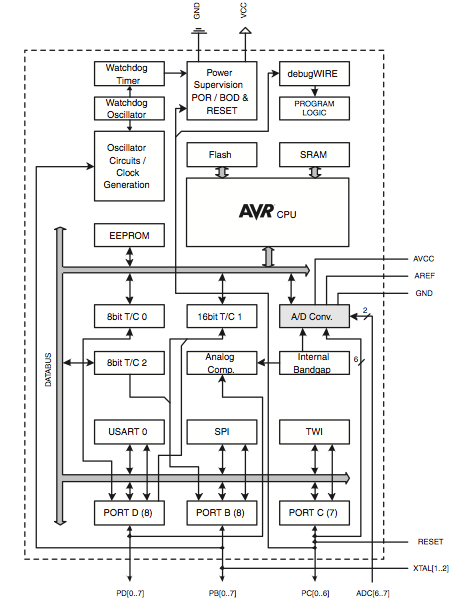
\includegraphics[height=12cm, width=10cm]{ArduinoBlockDiagram.png}
\caption{ATmega block diagram \protect\cite{BlockDiagram:URL}}
\label{Arduino Uno block diagram}
\end{figure}



\noindent \large The core implementation is divided into three main sections.

\section{Memory and registers}

In ATmega328, memory is divided into 3 main parts.
\subsection{Flash memory}
It is a non-volatile read only memory of 32 KB addressed by 15-bit addresses 0.5 KB of them are used by bootloader. it is used for storing the program. 

\subsection{SRAM (data memory)}
It is a volatile memory of 2 KB. It is divided into 32 registers, 64 I/O registers, 160 external I/O registers and internal SRAM.

\begin{figure}[h!]
\centering
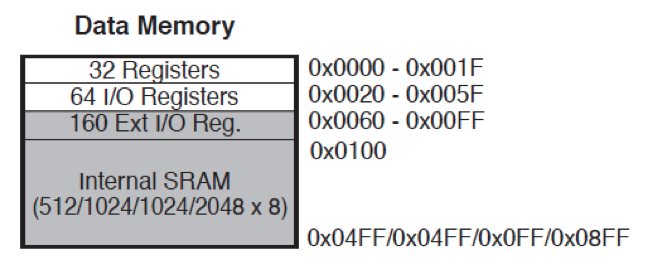
\includegraphics[height=4cm, width=9cm]{registers.png}
\caption{SRAM \protect\cite{WashUni:URL}}
\label{SRAM contents}
\end{figure}

\newpage

\noindent The following are special registers saved in the SRAM 

\subsubsection{Program Status Register(PSR)}

\begin{figure}[h!]
\centering
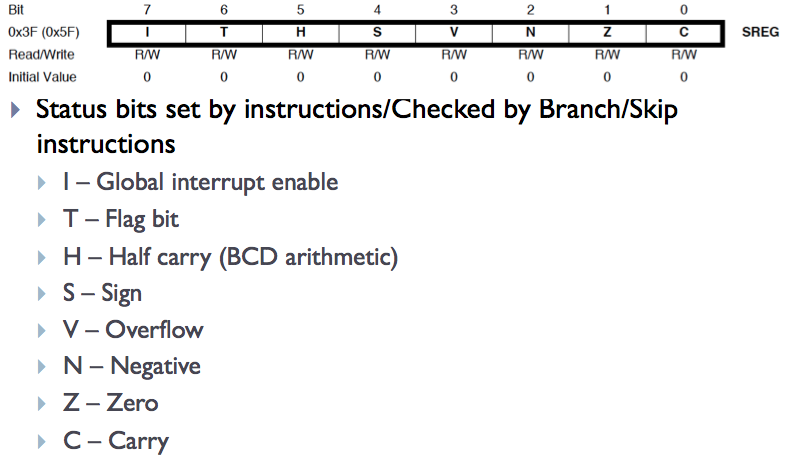
\includegraphics[height=7cm, width=12cm]{PSR.png}
\caption{Program Status Register \protect\cite{WashUni:URL}}
\label{Program Status Register}
\end{figure}

\subsubsection{Stack Pointer Register(SPR)}
It is a special register in I/O space [3E, 3D]

\subsubsection{RAMPX, RAMPY, RAMPZ}
Registers concatenated with the X-, Y-, and Z-registers enabling indirect addressing of the whole data space on MCUs with more than 64K bytes data space, and constant data fetch on MCUs with more than 64K bytes program space. 
				
\subsubsection{RAMPD}
Register concatenated with the Z-register enabling direct addressing of the whole data space on MCUs with more than 64K bytes data space. 
	
\subsubsection{EIND}
Register concatenated with the Z-register enabling indirect jump and call to the whole program space on MCUs with more than 64K words (128K bytes) program space. 
				
\subsection{EEPROM}
It is a long term data memory of 1 KB.


\section{Reading program process}
This is the process of receiving bytes of code and saving their values in the flash memory to be ready for execution.

\section{Program execution}

This section describes the process of executing the program saved in the flash memory. ATmega328 is based on the \href{http://www.atmel.com/images/doc0856.pdf}{8-bit AVR Instruction Set}. An instruction can be either 16 or 32 bits. The application reads two bytes to form a 16 bit instruction (most significant bits first). It executes the program by executing the following for every 2 bytes it reads. 

\noindent Implementation is divided into two parts

\subsection{Matching opcode}
To determine the operation to execute, Instruction should be matched with an opcode of a certain operation. Matching is done by performing bitwise operations on the instruction depending on the opcode. After matching with an opcode, bitwise operations are performed to extract the operands from the instruction. Then comes the next part of executing the matched instruction.
\noindent Instruction might match with a 32 bit opcode which requires reading the next two bytes to extract the operand.

\begin{figure}[h!]
\centering
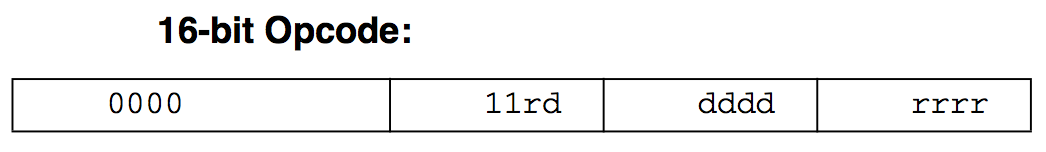
\includegraphics[height=1.5cm, width=10cm]{opcode.png}
\caption{ADD instruction opcode \protect\cite{opcode:URL}}
\label{Instruction opcode example}
\end{figure}

\newpage

\subsection{Executing Instruction}
After matching the instruction with an opcode, operation is executed depending on the opcode. Opcodes for all instructions and their operation are found in the \href{http://www.atmel.com/images/doc0856.pdf}{AVR Instruction Set documentation}.
